\subsubsection{Vorstellung des Amazon Dash Buttons}        
\label{sec:Vorstellung des Amazon Dash Buttons} 
Am 31.08.16 wurde der Amazon Dash Button offiziell in Deutschland exklusiv für Prime Mitglieder eingeführt (vgl. \cite{ONLINE.31.08.2016}).
Dabei handelt es sich um einem mit dem WLAN verbundenen Button, mit welchem sich zum Großteil Verbrauchsartikel per Knopfdruck bestellen lassen. Jeder Button wird mit einem Produkt verknüpft, das während des Einrichtens ausgewählt wird. Sollte nun das Produkt zur Neige gehen oder gar aufgebraucht sein, so kann der Nutzer den Button drücken und es wird sofort ein Bestellvorgang eingeleitet. Weitere Interaktion seitens des Nutzers ist dabei nicht notwendig.

\begin{figure}[!htb]
	\centering
	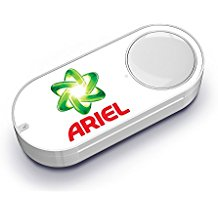
\includegraphics[scale=0.5]{Dash.jpg}
	\caption[Amazon Dash Button für Produkte von Ariel]{Amazon Dash Button für Produkte von Ariel,\\ Quelle: https://images-eu.ssl-images-amazon.com/images/I/41SMHhklQYL.\_AC\_US218\_.jpg}
\end{figure}

\subsubsection{Untersuchung des Amazon Dash Buttons}
\label{sec:Untersuchung des Amazon Dash Buttons}

\subsubsection{Verwendung des Amazon Dash Buttons im Projekt}
\label{sec:Verwendung des Amazon Dash Buttons im Projekt}
